%%% -*-LaTeX-*-

\chapter[A Mixed Real and Floating Point Solver]{A Mixed Real and Floating\\Point Solver}
\label{sec:fprock}
Reprinted from Proceedings of the 11th Annual NASA Formal Methods Symposium (NFM), pages 363-370, May 2019: "A Mixed Real and Floating-Point Solver" by Rocco Salvia, Laura Titolo, Marco A. Feli\'{u}, Mariano M. Moscato, C\'{e}sar A. Mu\~{n}oz and Zvonimir Rakamari\'c. Reprinted by permission.\\
https://doi.org/10.1007/978-3-030-20652-9\_25


\setupuuchapterbib
\uudummysection {Introduction}                              		{1}
\uudummysection {Solving Mixed Real/Floating-Point Formulas}		{2}
\uudummysection {Integrating FPRoCK in PRECiSA}       				{3}
\uudummysection {Conclusions}                      					{4}
\uudummytable   {Experimental results showing absolute round-off error bounds and execution time in seconds (best results in bold).}          					{5}
\uudummysection {References}                              			{5}

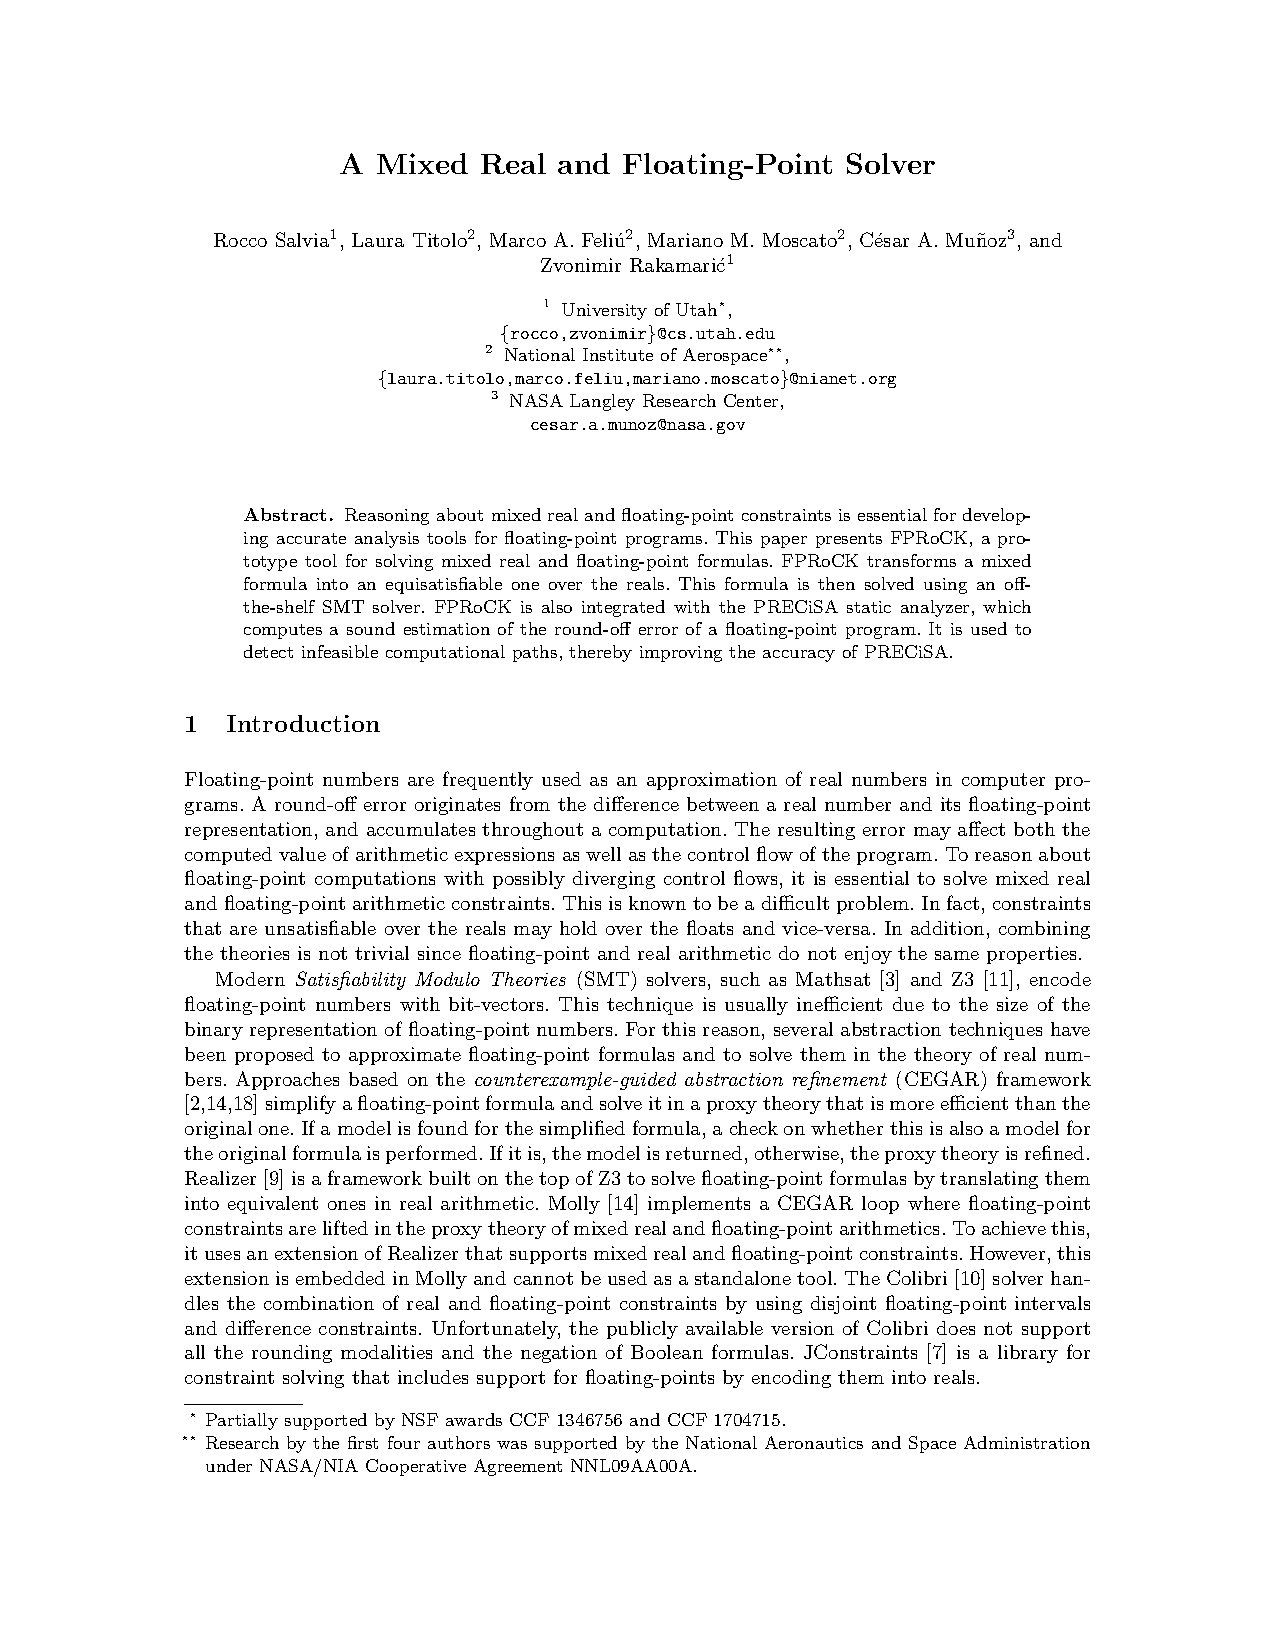
\includepdf[
	pages = -,          % want all document pages
	scale = 0.95,       % adjust to fit thesis page box
	pagecommand = {\pagestyle{plain}} % bare page numbers
]{fprock/main.pdf}

\bibliographystyle{plain}
\bibliography{main}

%\BibTeX{} entries themselves.
%\bibliographystyle{siam}
%\bibliography{refs}